\section{Värmeutveckling}

\textbf{
HAREC a.\ref{HAREC.a.2.7}\label{myHAREC.a.2.7}
}

\index{värmeutveckling}
\index{heat dissipation}

\subsection{Värmeledning}

\textbf{
HAREC a.\ref{HAREC.a.2.7.1}\label{myHAREC.a.2.7.1}
}

\index{värmeledning}
\index{heat transfer}
\index{termisk resistans}
\index{symbol!\(R_\Theta\) termisk resistans}
\index{omgivande temperatur}
\index{ambient temperature}
\index{symbol!\(T_A\) ambient temperature}
\index{elsäkerhet}
\index{kallödning}

Vi har tidigare betraktat Joules lag för effektutveckling i motstånd.
Det är dags att börja utveckla en lite mer komplett syn på värmeutveckling.
Ett motstånd som utvecklar 1~watt kommer stiga i temperatur till dess att
jämvikt uppstår mellan motståndets förmåga att avleda värme och
omgivningstemperaturen.

\emph{Termisk resistans} (eng. \emph{thermal resistance}) är ett mått på
hur bra ett material är på att leda värme. Den betecknas med symbolen \(R_\Theta\),
och anges i enheten kelvin per watt.
Temperaturen \(T_k\) för en komponent beror på medeleffekten \(P\) som den
producerar i värme, den termiska resistansen samt den \emph{omgivande temperaturen}
(eng. \emph{ambient temperature}) \(T_A\) enligt:

\(T_k = T_A + R_\Theta \cdot P\)

De termiska resistanserna för komponent, kylpasta, isolerskiva och kylfläns
kan summeras precis som resistanser för vanliga motstånd och det
sammanlagda värdet används sedan för att beräkna temperaturen på en
komponent eller för att dimensionera en kylfläns.

\subsection{Konvektion}
\textbf{
HAREC a.\ref{HAREC.a.2.7.2}\label{myHAREC.a.2.7.2}
}
\index{konvektion}
\index{kylfläns}
\index{heatpipe}

\emph{Konvektion} (eng. \emph{convection}) är när värme skapar ett
naturligt flöde i vätska eller gas, oftast luft. När luft värms upp 
vill den expandera, varvid densiteten sjunker och luften vill stiga uppåt.
Kallare luft strömmar då till och kan därmed kyla värmekällan. En stor
temperaturskillnad medför att konvektionen ökar och innebär därmed en bättre
kylning.

För exempelvis transistorer kan värmealstringen ske på en sådan liten yta att
konvektion från komponenten inte räcker för att kyla bort den producerade
värmen. Därför monterar man dem på en \emph{kylfläns} (eng.
\emph{heat sink}) som fördelar värmen över en större yta så att verkan av
konvektion ökar.

En effektiv metod för att transportera värme är via en så kallad \emph{heat pipe}.
Det är ett rör innehållande en vätska som förångas vid en temperatur strax över
rumstemperatur och som då effektivt leder överskottsvärme till ett plats där den kan
kylas bort. Heat pipe används numera ofta i datorer och solfångare.

Om värme produceras på en liten yta kan man behöva hjälpa konvektionen, vilket
ibland kallas för \emph{forcerad konvektion} (eng. \emph{forced convection}).
Med hjälp av en fläkt blåses luft mot eller sugs förbi kylflänsen vilket ökar
värmeutbytet. Eftersom fläktar skapar oljud brukar man försöka anpassa
fläktens varvtal i förhållande till temperaturen, men även en variation av
varvtal kan uppfattas som störande. Andra åtgärder för att minska ljudnivån
är att skapa släta ytor för luften så det inte bildas luftvirvlar eller att 
styra in- och utgående luftflöde med bafflar.

Ett problem som kan uppstå är att utrustning som är gjord för självkonvektion
blir placerad eller monterad så att luft inte kan flöda fritt runt
utrustningen. Detta kan leda till överhettning på motsvarande sätt som när
en fläkt för forcerad kylning går sönder. Dålig termisk kontakt mellan
transistor och kylfläns är ett annat exempel på hur dålig värmeledning skapar
problem med överhettning.

\subsection{Värmealstring}
\textbf{
HAREC a.\ref{HAREC.a.2.7.4}\label{myHAREC.a.2.7.4}
}
\index{värmealstring}

\emph{Värmealstring} kan ske på fler ställen än i motstånd. Lite förenklat
kan man säga att alla komponenter har förluster som producerar värme. Genom
lämpligt val av komponenter och korrekt dimensionering kan vi undvika att
producera onödiga värmeförluster. Kraftaggregat och effektsteg är exempel
på apparater där det går större strömmar vilka ofrånkomligen också alstrar
mera värme. Lägre förluster skapar man genom att helt enkelt ha bättre
ledningsförmåga, lägre resistans.

Även halvledare skapar värme, och även här gäller Joules lag med spänning
gånger ström. I exempelvis ett effektsteg kommer transistorn utveckla en
effekt motsvarande spänningen över transistorn gånger strömmen genom den. 
Onödigt hög spänning och ström skapar högre värmeutveckling, vilket är en 
anledning till att man gärna undviker slutsteg som arbetar i klass A till fördel för
slutsteg som arbetar i klass AB, B eller C.

Bristande värmeavledning leder ofta till katastrofala fel, som till exempel
sönderbrända motstånd och transistorer. Även ledare kan brinna av när man
har för liten ledararea, och därmed för hög resistans för den ström som
ska gå genom den. Av det skälet finns dimensioneringsregler, till exempel
krav på minsta arean av koppar i ledare, helt enkelt för att det inte ska
uppstå brand.

En annan effekt av värmeledning är att det kan ibland vara svårt att löda
på kretskort, framför allt vid ledare som går mot stora kopparytor som
har en relativt god värmeledningsförmåga. Ibland konstruerar man små mönster
''thermals'' runt sådana lödpunkter för att minska värmeavledningen.
Ett effektivt sätt att kunna löda och framförallt löda av från sådana
kort är att man förvärmer hela kretskortet eller området runt om
lödpunkten. Då kommer temperaturskillnaden mellan lödpennans spets och
omgivningen att minska och det krävs inte lika stor effekt för att få
upp lödpunkten i rätt temperatur för att kunna genomföra lödningen med god
\emph{vätning} och därmed undvika att det bildas en kallödning.

\subsection{Värme i transistor}
\textbf{
HAREC a.\ref{HAREC.a.2.7.3}\label{myHAREC.a.2.7.3}
}

För att förstå värmealstring i en transistor börjar vi med att tänka oss
att vi har en transistor med 12~V matningsspänning. Vi låter den generera en
sinussignal med topp-till-topp-värdet \(10\ V_{pp}\) in i en 50~ohms last.
Vad är effektförlusten i transistorn?

\begin{figure}[ht]
\begin{center}
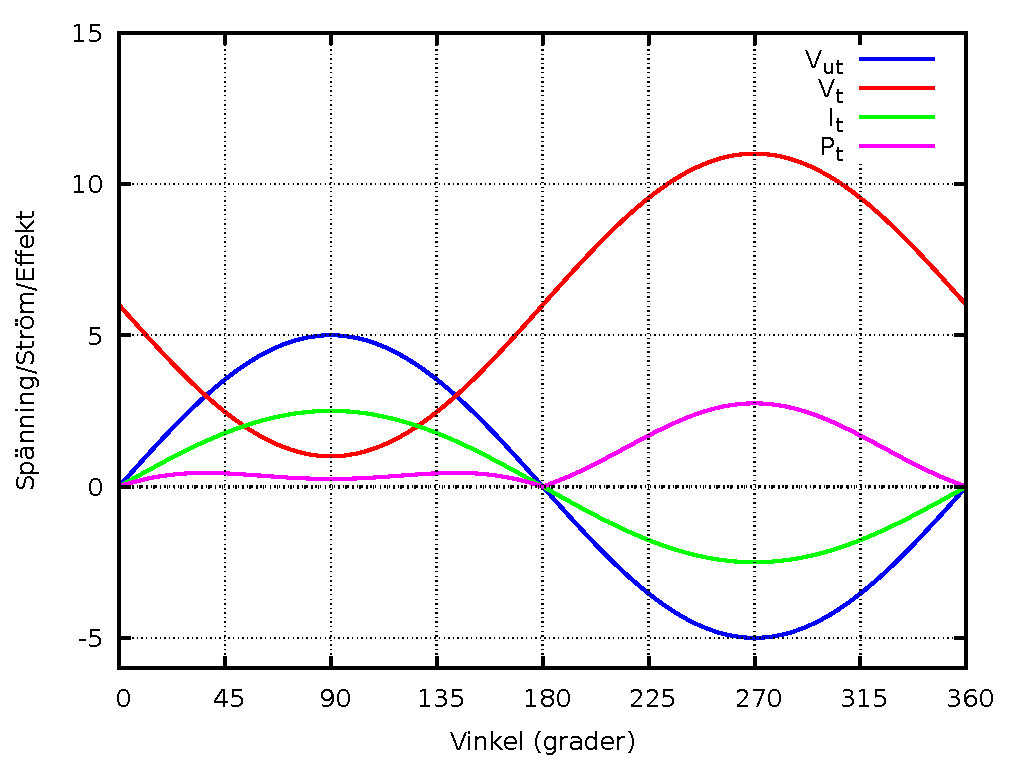
\includegraphics[width=7cm]{images/power1.pdf}
\caption{Utspänning $U_{ut}$, transistorspänning $U_t$, transistorström $I_t$ och transistoreffekt $P_t$ varierar med vinkeln hos sinussignalen för resistiv last.}
\label{fig:power1}
\end{center}
\end{figure}

I bild \ref{fig:power1} ser vi utsignalen \(U_{ut}\) som en sinussignal med amplituden
\(10\ V_{pp}\). Transistorn har en vilospänning på 6~V
för att få marginal mot \(0\ V\) och \(+12\ V\). Spänningen \(U_t\) varierar
mellan \(1\ V\) och \(11\ V\). I utgångslastens resistor alstras en ström \(I_t\) som är proportionerlig mot spänningen
\(U_{ut}\) på utgången. Effekten för transistorn \(P_t\) är absolutvärdet av strömmen gånger spänningen enligt Joules lag. 

\(P_t = \lvert U_t \cdot I_t \rvert\) 

Den observante ser att effekten är signifikant högre för andra halvan av kurvan, då man har både
hög spänning och hög ström.
